\documentclass{article}
\usepackage{tikz}

% Definition of circles
\def\firstcircle{(0,0) circle (1.8cm)}
\def\secondcircle{(2,0) circle (1.8cm)}
\def\thirdcircle{(1,-2) circle (1.8cm)}

\colorlet{circle edge}{blue!50}
\colorlet{circle area}{blue!20}

\tikzset{filled/.style={fill=circle area, draw=circle edge, thick},
	outline/.style={draw=circle edge, thick}}



\usepackage{geometry}

\setlength{\parindent}{0pt}
\setlength{\parskip}{5pt}

\title{CORE111 Logical Problem Solving\\Homework 4}
\author{My Name}

\begin{document}
\maketitle

\section{Fallacies}

(a) Assuming that his conclusion is "American needs defense" (which would imply America needs B1), he is trying to form a relation between being peaceful and needing a defense.(The fallacy of cause) He also misses the point when asked about effectiveness of the plane to support his argument. (Missing the Point)

(b) Formal fallacy because if his fingerprint weren't found it could be that he either didn't commit the crime or was wearing gloves or the negation of etc 

(c) circular reasoning

(d) Slippery slope; From frustrating middle management to worker and failing the company

(e) Circular Reasoning

(f) Slippery slope

(g) no Fallacy 

(h) it can be called a hasty generalization because finding new ways our mind relates to our bodies do not in any way imply the word soul won't be used

(i) Formal Fallacy

(j) he has no evidence in favor or against the claim but still he has decided to go in favor of it.(Burden of proof)

\section{Categorical Syllogisms}

(a)  From premises we get. \\

\fbox{%
		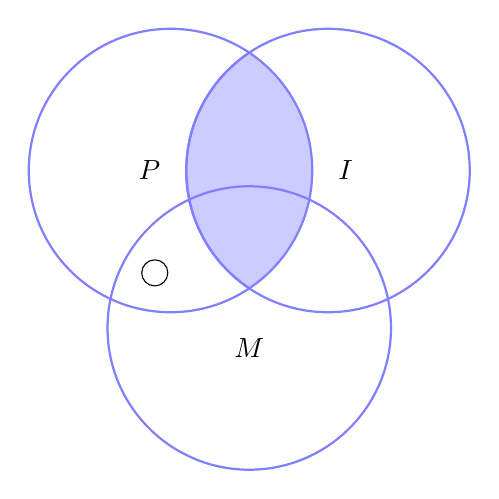
\begin{tikzpicture}
		\begin{scope}
		\clip \firstcircle;
		\draw[filled] \secondcircle;
		\clip \thirdcircle;
		\end{scope}
		\node[draw,circle] (b) at (-.2,-1.3) {};
		\draw[outline] \firstcircle node[left] {$P$};
		
		\draw[outline] \secondcircle node[right] {$I$};
		\draw[outline] \thirdcircle node[below] {$M$};
		\end{tikzpicture}
	}\\
Conclusion requires: \\
\fbox{%
		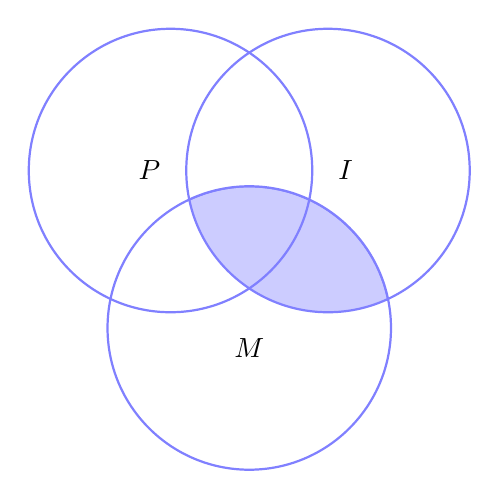
\begin{tikzpicture}
		\begin{scope}
		\clip \secondcircle;
		
		\clip \thirdcircle;
		\draw[filled] \thirdcircle;
		
		\end{scope}
		\draw[outline] \firstcircle node[left] {$P$};
		\draw[outline] \secondcircle node[right] {$I$};
		\draw[outline] \thirdcircle node[below] {$M$};
		
		\end{tikzpicture}
	}\\
The conclusion is invalid\\

(b) From premises we get. \\

\fbox{%
		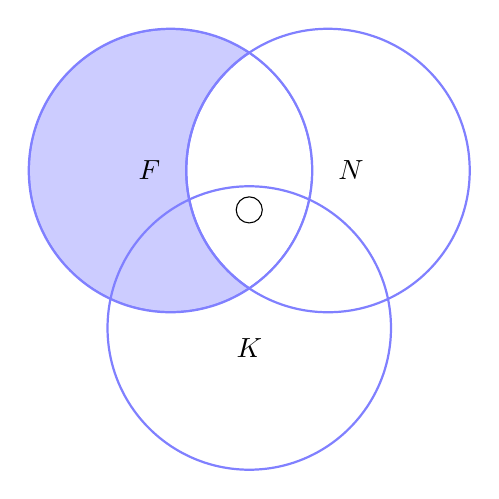
\begin{tikzpicture}
		\begin{scope}
			\clip \firstcircle;
			\draw[filled, even odd rule] \secondcircle
			\firstcircle;
			\end{scope}
		\draw[outline] \firstcircle node[left] {$F$};
		
		\draw[outline] \secondcircle node[right] {$N$};
		\draw[outline] \thirdcircle node[below] {$K$};
		\node[draw,circle] (b) at (1,-0.5) {};
		\end{tikzpicture}
	}
	\fbox{%
		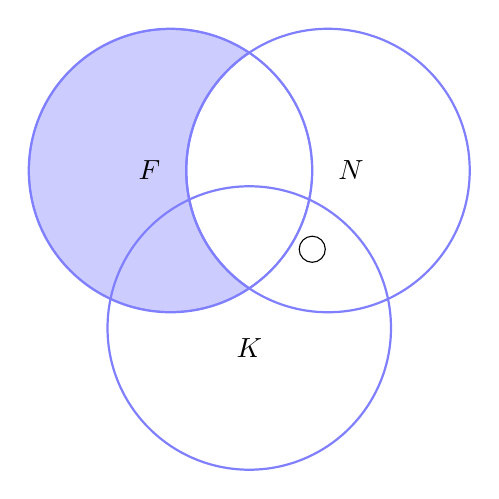
\begin{tikzpicture}
		\begin{scope}
			\clip \firstcircle;
			\draw[filled, even odd rule] \secondcircle
			\firstcircle;
			\end{scope}
		\draw[outline] \firstcircle node[left] {$F$};
		
		\draw[outline] \secondcircle node[right] {$N$};
		\draw[outline] \thirdcircle node[below] {$K$};
		\node[draw,circle] (b) at (1.8,-1) {};
		\end{tikzpicture}
	}\\
Conclusion requires any of these: \\
\fbox{%
		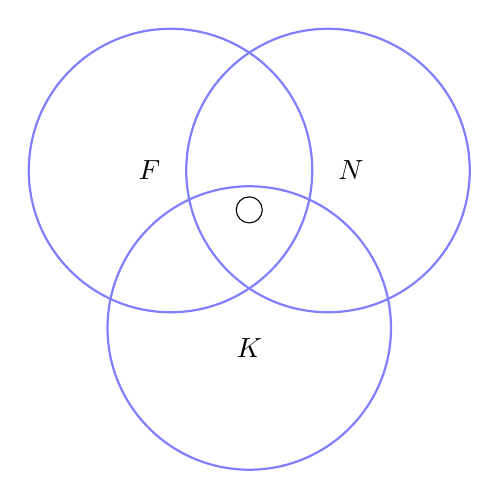
\begin{tikzpicture}
		\draw[outline] \firstcircle node[left] {$F$};
		\draw[outline] \secondcircle node[right] {$N$};
		\draw[outline] \thirdcircle node[below] {$K$};
		\node[draw,circle] (b) at (1,-0.5) {};
		\end{tikzpicture}
	}
	\fbox{%
		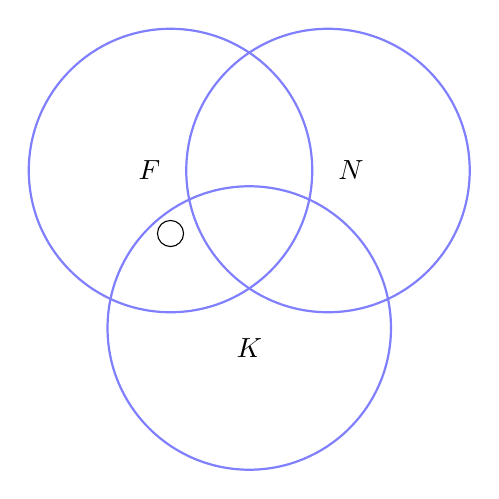
\begin{tikzpicture}
		\draw[outline] \firstcircle node[left] {$F$};
		\draw[outline] \secondcircle node[right] {$N$};
		\draw[outline] \thirdcircle node[below] {$K$};
		\node[draw,circle] (b) at (0,-0.8) {};
		\end{tikzpicture}
	}\\
The conclusion is invalid because not both cases from premises are satisfied by either of the possible conclusion\\
(c)
  From premises we get. \\

\fbox{%
		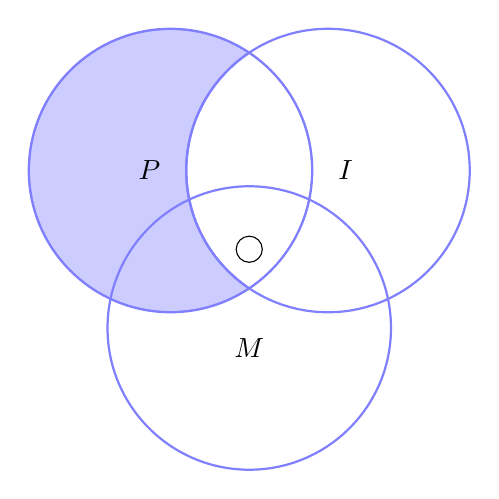
\begin{tikzpicture}
		\begin{scope}
			\clip \firstcircle;
			\draw[filled, even odd rule] \secondcircle
			\firstcircle;
			\end{scope}
		\draw[outline] \firstcircle node[left] {$P$};
		
		\draw[outline] \secondcircle node[right] {$I$};
		\draw[outline] \thirdcircle node[below] {$M$};
		\node[draw,circle] (b) at (1,-1) {};
		\end{tikzpicture}
	}\\
Conclusion requires either of: \\
\fbox{%
		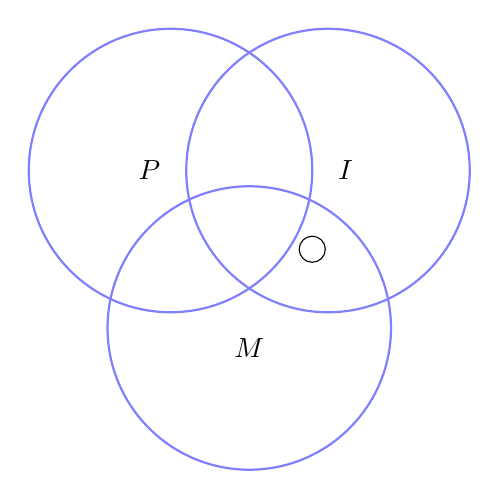
\begin{tikzpicture}

		\draw[outline] \firstcircle node[left] {$P$};
		\draw[outline] \secondcircle node[right] {$I$};
		\draw[outline] \thirdcircle node[below] {$M$};
		\node[draw,circle] (b) at (1.8,-1) {};
		
		\end{tikzpicture}
	}
\fbox{%
		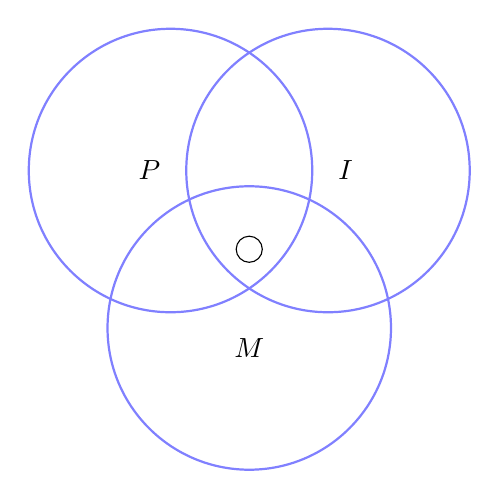
\begin{tikzpicture}

		\draw[outline] \firstcircle node[left] {$P$};
		\draw[outline] \secondcircle node[right] {$I$};
		\draw[outline] \thirdcircle node[below] {$M$};
		\node[draw,circle] (b) at (1,-1) {};
		
		\end{tikzpicture}
	}\\
The conclusion is valid\\
(d) From premises we get. \\

\fbox{%
		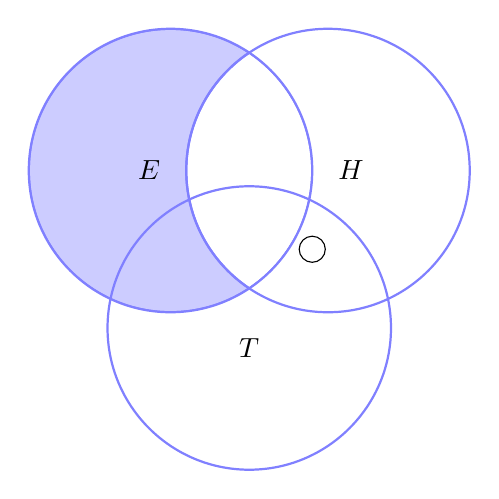
\begin{tikzpicture}
		\begin{scope}
			\clip \firstcircle;
			\draw[filled, even odd rule] \secondcircle
			\firstcircle;
			\end{scope}
		\draw[outline] \firstcircle node[left] {$E$};
		
		\draw[outline] \secondcircle node[right] {$H$};
		\draw[outline] \thirdcircle node[below] {$T$};
		\node[draw,circle] (b) at (1.8,-1) {};
		\end{tikzpicture}
	}
	\fbox{%
		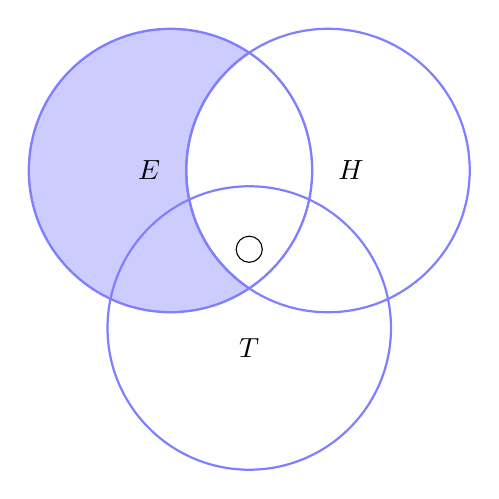
\begin{tikzpicture}
		\begin{scope}
			\clip \firstcircle;
			\draw[filled, even odd rule] \secondcircle
			\firstcircle;
			\end{scope}
		\draw[outline] \firstcircle node[left] {$E$};
		
		\draw[outline] \secondcircle node[right] {$H$};
		\draw[outline] \thirdcircle node[below] {$T$};
		\node[draw,circle] (b) at (1,-1) {};
		\end{tikzpicture}
	}\\
Conclusion requires: \\
\fbox{%
		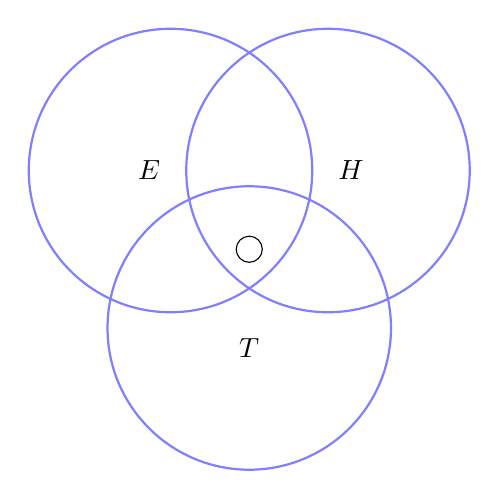
\begin{tikzpicture}

		\draw[outline] \firstcircle node[left] {$E$};
		\draw[outline] \secondcircle node[right] {$H$};
		\draw[outline] \thirdcircle node[below] {$T$};
		\node[draw,circle] (b) at (1,-1) {};
		
		\end{tikzpicture}
	}
	\fbox{%
		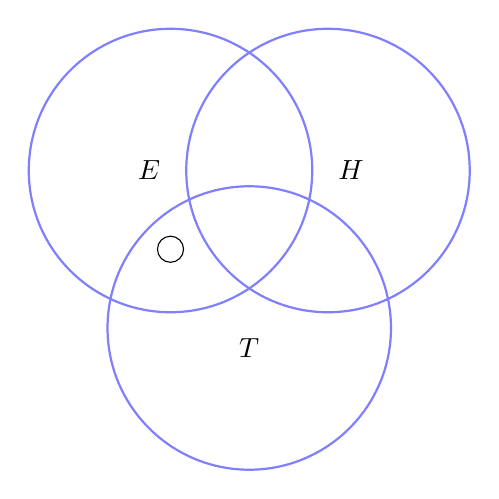
\begin{tikzpicture}

		\draw[outline] \firstcircle node[left] {$E$};
		\draw[outline] \secondcircle node[right] {$H$};
		\draw[outline] \thirdcircle node[below] {$T$};
		\node[draw,circle] (b) at (0,-1) {};
		
		\end{tikzpicture}
	}\\
The conclusion is invalid \\
(e) From premises we get. \\

\fbox{%
		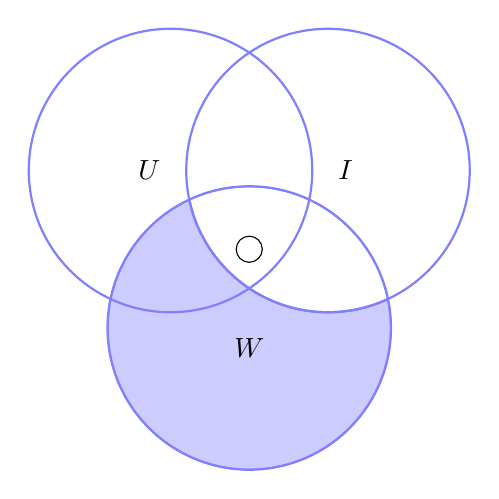
\begin{tikzpicture}
		\begin{scope}
			\clip \thirdcircle;
			\draw[filled, even odd rule] \secondcircle
			\thirdcircle;
			\end{scope}
		\node[draw,circle] (b) at (1,-1) {};
		\draw[outline] \firstcircle node[left] {$U$};
		
		\draw[outline] \secondcircle node[right] {$I$};
		\draw[outline] \thirdcircle node[below] {$W$};
		\end{tikzpicture}
	}\fbox{%
		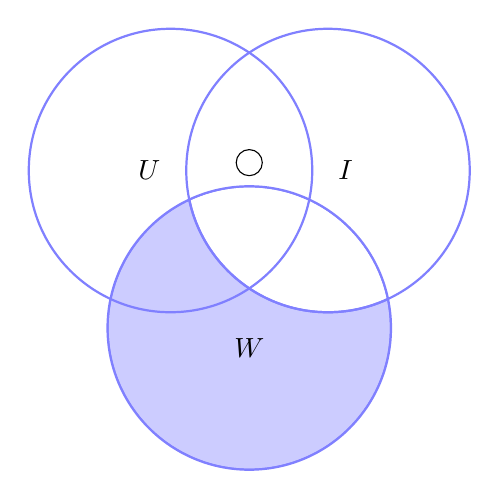
\begin{tikzpicture}
		\begin{scope}
			\clip \thirdcircle;
			\draw[filled, even odd rule] \secondcircle
			\thirdcircle;
			\end{scope}
		\node[draw,circle] (b) at (1,0.1) {};
		\draw[outline] \firstcircle node[left] {$U$};
		
		\draw[outline] \secondcircle node[right] {$I$};
		\draw[outline] \thirdcircle node[below] {$W$};
		\end{tikzpicture}
	}\\
Conclusion requires: \\
\fbox{%
		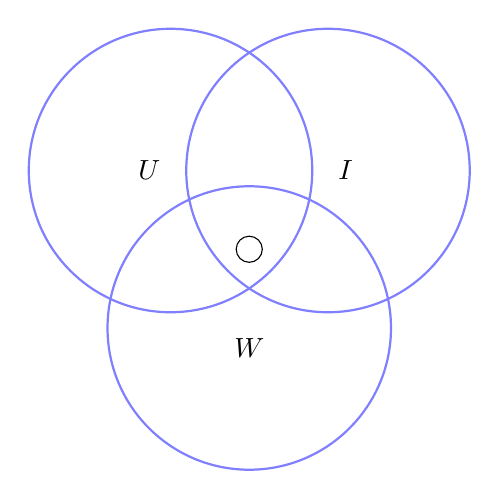
\begin{tikzpicture}

		\draw[outline] \firstcircle node[left] {$U$};
		\draw[outline] \secondcircle node[right] {$I$};
		\draw[outline] \thirdcircle node[below] {$W$};
		\node[draw,circle] (b) at (1,-1) {};
		
		\end{tikzpicture}
	}
	\fbox{%
		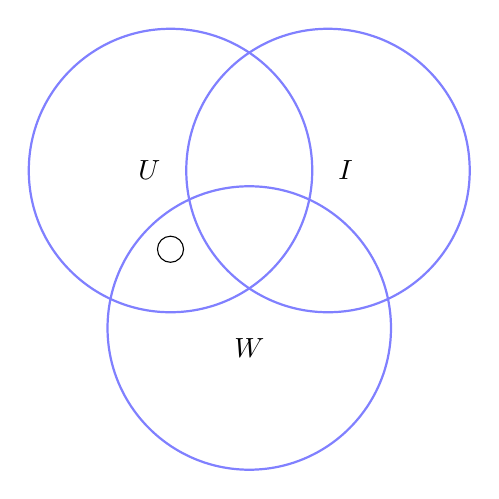
\begin{tikzpicture}

		\draw[outline] \firstcircle node[left] {$U$};
		\draw[outline] \secondcircle node[right] {$I$};
		\draw[outline] \thirdcircle node[below] {$W$};
		\node[draw,circle] (b) at (0,-1) {};
		
		\end{tikzpicture}
	}\\
The conclusion is invalid\\

\end{document}